\documentclass[12pt]{article}

% 基础宏包
\usepackage{graphicx}  % 插入图片
\usepackage[english]{babel}  % 英语语言支持
% \usepackage[UTF8]{ctex}  % 如果不需要中文，可以注释掉这一行

% 数学宏包
\usepackage{amsmath}  % 数学排版增强
\usepackage{amsfonts} % 数学字体

% 图表相关
\usepackage{float}    % 浮动体控制 [H] 选项
\usepackage{tikz}     % 绘图
\usepackage{pgfplots} % 函数绘图
\pgfplotsset{compat=1.18} % 设置pgfplots兼容性

% 页面设置
\usepackage{geometry}
\geometry{
  a4paper,
  left=2cm,
  right=2cm,
  top=2cm,
  bottom=2cm
}

% 版式设置
\usepackage{fancyhdr}    % 页眉页脚
\usepackage{lastpage}    % 最后一页引用
\usepackage{multicol}    % 多栏排版
\usepackage{tabularx}    % 表格增强

% 文本修饰
\usepackage{ulem}        % 下划线等
\usepackage{enumitem}    % 列表样式
\usepackage{titlesec}    % 标题样式
\usepackage[export]{adjustbox} % 图片对齐

% 颜色
\usepackage{color}       % 颜色支持

\linespread{1.5}         % 1.5倍行距

\title{Lab 4}
\author{Emilien Zhang}
\date{26 May 2026}

\begin{document}

\maketitle

\section*{Problem 1}

\subsection*{(a)}




Given:
\[
h[n] = 2\delta[n+1] - 2\delta[n-1], \quad x[n] = \delta[n] + \delta[n-2]
\]

From the convolution definition:
\[
y[n] = h[n] * x[n] = \sum_{k=-\infty}^{\infty} h[k] x[n-k]
\]

Since \(h[k]\) is nonzero only at \(k = -1\) and \(k = 1\):
\[
y[n] = 2x[n+1] - 2x[n-1]
\]

Substituting \(x[n] = \delta[n] + \delta[n-2]\):
\[
y[n] = 2\bigl(\delta[n+1] + \delta[n-1]\bigr) - 2\bigl(\delta[n-1] + \delta[n-3]\bigr) = 2\delta[n+1] - 2\delta[n-3]
\]

Thus:
\[
\boxed{y[-1] = 2,\quad y[3] = -2}
\]

\begin{figure}[H]
  \centering
  
\includegraphics[width=0.8\textwidth]{1.jpg}
  
\end{figure}


The starting indices are \(n_h = -1\) and \(n_x = 0\), so the output starting index is \(n_y = n_h + n_x = -1\). The output length is \(N_h + N_x - 1 = 3 + 3 - 1 = 5\). Hence the output indices are:
\[
\mathbf{ny} = [-1,\;0,\;1,\;2,\;3]
\]

\subsection*{(b)}

Let:
\[
h[n] = \delta[n-a] + \delta[n-b], \quad x[n] = \delta[n-c] + \delta[n-d]
\]

The convolution result is:
\[
y[n] = \delta[n-(a+c)] + \delta[n-(a+d)] + \delta[n-(b+c)] + \delta[n-(b+d)]
\]

Therefore, the set of indices where \(y[n]\) is nonzero is:
\[
\{a+c,\; a+d,\; b+c,\; b+d\}
\]

The range of output indices is:
\[
\mathbf{ny} = [a+c,\; b+d]
\]

Verification: when \(a=0,\; b=N-1,\; c=0,\; d=M-1\),
\[
\text{output length} = (b+d) - (a+c) + 1 = (N-1 + M-1) - 0 + 1 = M + N - 1
\]
which matches the convolution length formula.

\begin{figure}[H]
  \centering
  
\includegraphics[width=0.8\textwidth]{2.jpg}
  
\end{figure}

Let us verify the indexing formula with a concrete example.  
Choose \(a = 0\), \(b = 2\), \(c = 1\), \(d = 4\). Then:

\[
h[n] = 1 \quad \text{for } n \in \{0,1,2\}, \qquad
x[n] = 1 \quad \text{for } n \in \{1,2,3,4\}.
\]

The convolution \(y[n] = h[n] * x[n]\) yields a sequence that is nonzero for:

\[
n \in [a+c,\; b+d] = [0+1,\; 2+4] = [1,\; 6].
\]

The length of \(y\) is:

\[
(b - a + 1) + (d - c + 1) - 1 = 3 + 4 - 1 = 6,
\]

which matches the number of indices from \(1\) to \(6\) inclusive.  

Thus, the output index vector is:

\[
\mathbf{ny} = [1,\;2,\;3,\;4,\;5,\;6].
\]

This confirms that for any \(a,b,c,d\), the correct time indices for the convolution result are \(\mathbf{ny} = [a+c,\; b+d]\).

\subsection*{(c)}

Given:
\[
x[n] = \left(\frac12\right)^{n-2} u[n-2], \quad h[n] = u[n+2]
\]

Truncation:
\begin{itemize}
    \item \(x[n]\) is stored for \(0 \leq n \leq 24\)
    \item \(h[n]\) is stored for \(0 \leq n \leq 14\)
\end{itemize}

The starting indices of the complete signals are \(n_x = 2\) and \(n_h = -2\), so the complete output starting index is \(n_y = 0\).

Because \(h[n]\) is truncated for \(n < 0\) (losing \(h[-2]\) and \(h[-1]\)), the first 2 samples of the convolution result are invalid. Additionally, because \(x[n]\) is truncated for \(n > 24\), the tail samples are also invalid. Using the result from part (b), the valid output index range within the truncated interval is:
\[
\mathbf{ny\_valid} = [0,\; 38]
\]

Thus, in the output returned by `conv`, samples starting from the 3rd sample are valid. The number of invalid tail samples depends on the tolerance for truncation error.


\begin{figure}[H]
  \centering
  
\includegraphics[width=0.8\textwidth]{3.jpg}
  
\end{figure}
\subsection*{(d)}

Given:
\[
h[n] = (0.9)^n \bigl(u[n] - u[n-10]\bigr), \quad x[n] = \cos(n^2) \sin\left(\frac{2\pi n}{5}\right)
\]

Compute \(y[n] = h[n] * x[n]\) for \(0 \leq n \leq 99\) directly using the convolution definition. The length of \(h[n]\) is \(P = 10\) and the length of \(x[n]\) is \(N = 100\), so the output length is \(N + P - 1 = 109\). Plot \(y[n]\) versus \(n\) using a stem plot.


\begin{figure}[H]
  \centering
  
\includegraphics[width=0.8\textwidth]{4.jpg}
  
\end{figure}
\subsection*{(e)}

Use the overlap-add method for block convolution. Choose block length \(L = 50\) and split \(x[n]\) into two blocks:
\[
x_0[n] = x[n],\quad 0 \leq n \leq 49, \qquad x_1[n] = x[n+50],\quad 0 \leq n \leq 49
\]

Compute the convolutions separately:
\[
y_0[n] = h[n] * x_0[n], \quad y_1[n] = h[n] * x_1[n]
\]

Each output block has length \(L + P - 1 = 59\). The overall output is:
\[
y[n] = y_0[n] + y_1[n - 50]
\]
where \(k = 50\) is the offset.

Add \(y_0[n]\) and the shifted \(y_1[n-50]\). In the overlap region (\(n = 50\) to \(n = 58\)), both blocks are nonzero and must be summed. This result is identical to the direct convolution obtained in part (d).


\begin{figure}[H]
  \centering
  
\includegraphics[width=0.8\textwidth]{5.jpg}
  
\end{figure}

\section*{Problme 2}

\subsection*{(a)}

Three 1D low-pass filters are designed with the same cutoff frequency \(w_c = 0.4\pi\):

\begin{enumerate}
    \item \textbf{Filter 1 (Butterworth, IIR)}: order \(n_1 = 10\), designed using the Butterworth method. This filter has an infinite impulse response.
    \item \textbf{Filter 2 (FIR)}: order \(n_2 = 4\), designed using the Parks-McClellan algorithm. The frequency bands are:
    \[
    [0,\; w_c-0.04] \text{ with gain } 1,\quad [w_c+0.04,\; 1] \text{ with gain } 0
    \]
    \item \textbf{Filter 3 (FIR)}: order \(n_3 = 12\), designed using the same method with identical band specifications.
\end{enumerate}

The coefficients are denoted as \((b_1, a_1)\) for Filter 1, \((b_2, a_2)\) for Filter 2, and \((b_3, a_3)\) for Filter 3. For FIR filters, \(a_2 = a_3 = 1\).

\subsection*{(b)}

The frequency response \(H(e^{j\omega})\) of each filter is computed using the \texttt{freqz} function with 512 frequency points between \(0\) and \(\pi\).

For each filter, both magnitude response \(|H(e^{j\omega})|\) and phase response \(\angle H(e^{j\omega})\) are plotted against normalized frequency \(\omega/\pi\).

\begin{figure}[H]
  \centering
  
\includegraphics[width=0.8\textwidth]{6.jpg}
  \end{figure}

Observations:
\begin{itemize}
    \item All three filters have a cutoff frequency approximately at \(0.4\pi\), as specified.
    \item Filters 2 and 3 (FIR) exhibit \textbf{linear phase} — their phase responses are straight lines.
    \item Filter 1 (Butterworth, IIR) exhibits \textbf{nonlinear phase}.
\end{itemize}

\subsection*{(c)}

The step response of each filter is computed for \(0 \leq n \leq 20\) using the \texttt{filter} function. The step response is the output when the input is a unit step \(u[n]\).

For each step response, the overshoot is calculated as:
\[
\text{overshoot} = \max(y[n]) - y[\infty]
\]
where \(y[\infty]\) is the steady-state value (the last sample).

Results:
\begin{itemize}
    \item Filter 1 (Butterworth) has the largest overshoot.
    \item Filter 2 (FIR, order 4) has moderate overshoot.
    \item Filter 3 (FIR, order 12) has the smallest overshoot.
\end{itemize}

Large overshoot indicates ringing artifacts, which can lead to undesirable distortions in filtered images.

\begin{figure}[H]
   \centering
    
\includegraphics[width=0.8\textwidth]{7.jpg}
\end{figure}

\subsection*{(d)}

The 16th column of the image, denoted \(x_{16}[m]\) for \(0 \leq m \leq 31\), is extracted and filtered using Filter 1.

Since MATLAB's \texttt{filter} function implements causal filtering, a special technique is required to achieve noncausal filtering:
\begin{enumerate}
    \item Append \(d\) zeros to the end of the input signal, where \(d\) is the filter delay (half the filter order).
    \item Apply \(\texttt{filter}(b_1, a_1, \cdot)\) to the zero-padded signal.
    \item Take the last \(M\) samples (\(M = 32\)) as the noncausal filtering result.
\end{enumerate}

The original signal \(x_{16}[m]\) and the filtered output \(y_{16}[m]\) are plotted on the same axes. The discontinuities in the original signal align with smoothed transitions in the filtered signal, confirming that no delay or advance is introduced.

\begin{figure}[H]
  \centering
    
\includegraphics[width=0.8\textwidth]{8.jpg}
\end{figure}

\subsection*{(e)}

The same procedure from part (d) is repeated for Filter 2 and Filter 3. The delay parameters are:
\[
d_2 = \frac{4}{2} = 2,\qquad d_3 = \frac{12}{2} = 6
\]

All three filter outputs are plotted together with the original signal \(x_{16}[m]\). All three filters produce smooth transitions without positional shifts. The higher-order FIR filter (order 12) produces the most smoothing.

\begin{figure}[H]
  \centering
    
\includegraphics[width=0.8\textwidth]{9.jpg}
\end{figure}



\subsection*{(f)}

A function \(\texttt{filt2d}(b, a, d, x)\) is written to perform separable noncausal 2D filtering on an image.

Algorithm:
\begin{enumerate}
    \item \textbf{Column filtering}: For each column of the input image \(x\) (size \(M \times N\)), append \(d\) zeros, apply \(\texttt{filter}(b, a, \cdot)\), and take the last \(M\) samples. Store the result in an intermediate matrix \(z\).
    \item \textbf{Row filtering}: For each row of \(z\), append \(d\) zeros, apply \(\texttt{filter}(b, a, \cdot)\), and take the last \(N\) samples. Store the result in the output matrix \(y\).
\end{enumerate}

The function returns \(y\) with the same dimensions as \(x\). The column-then-row order ensures separable 2D filtering, and zero-padding guarantees noncausal behavior.

\subsection*{(g)}

The original image \(x\) is filtered using all three filters by calling \(\texttt{filt2d}\) with their respective coefficients:
\[
y_1 = \texttt{filt2d}(b_1, a_1, d_1, x),\quad
y_2 = \texttt{filt2d}(b_2, a_2, d_2, x),\quad
y_3 = \texttt{filt2d}(b_3, a_3, d_3, x)
\]

The images are displayed using a grayscale colormap and scaled by 64. The filtered images appear smoother than the original, and the center of the "plus" symbol remains at the same location in all images, confirming that no positional shift has occurred.

\begin{figure}[H]
  \centering
    
\includegraphics[width=1\textwidth]{10.jpg}
\end{figure}

\subsection*{(h)}

The three filters are compared based on distortion introduced to the image.

Observations:
\begin{itemize}
    \item Filter 1 (Butterworth, IIR) produces the most distortion. The "plus" symbol loses symmetry, and ringing artifacts appear near edges.
    \item Filter 2 (FIR, order 4) produces less distortion. The image remains symmetric but is somewhat blurred.
    \item Filter 3 (FIR, order 12) produces the least distortion, with good symmetry and minimal ringing.
\end{itemize}

The primary cause of distortion is \textbf{nonlinear phase}. Filter 1 has nonlinear phase, meaning different frequency components experience different delays, destroying the symmetry of the image. Filters 2 and 3 have linear phase, preserving symmetry.

Conclusion: For image processing applications, linear phase filters (FIR) are preferred over nonlinear phase filters (IIR).

\section*{Problme 3}

\subsection*{(a)}

Given DTFS coefficients for a periodic signal with fundamental period \(N = 5\):
\[
a_0 = 1,\quad a_2 = a_{-2}^* = e^{j\pi/4},\quad a_4 = a_{-4}^* = 2e^{j\pi/3}
\]

For a real-valued signal, the DTFS coefficients satisfy the conjugate symmetry condition:
\[
a_k = a_{-k}^*
\]

Since \(a_2 = a_{-2}^*\), \(a_4 = a_{-4}^*\), and \(a_0\) is real, the signal \(x[n]\) is predicted to be \textbf{purely real}.

\subsection*{(b)}

Using the conjugate symmetry property \(a_{-k} = a_k^*\) and the periodicity \(a_{N-k} = a_k^*\), the coefficients \(a_0\) through \(a_4\) are:

\[
\begin{aligned}
a_0 &= 1 \\
a_1 &= 0 \quad (\text{not specified, therefore zero}) \\
a_2 &= e^{j\pi/4} = \cos(\pi/4) + j\sin(\pi/4) = \frac{\sqrt{2}}{2} + j\frac{\sqrt{2}}{2} \\
a_3 &= a_{-3}^* = a_2^* = e^{-j\pi/4} = \frac{\sqrt{2}}{2} - j\frac{\sqrt{2}}{2} \\
a_4 &= 2e^{j\pi/3} = 2\left(\cos(\pi/3) + j\sin(\pi/3)\right) = 1 + j\sqrt{3}
\end{aligned}
\]

Thus the coefficient vector is:
\[
\mathbf{a} = [a_0,\; a_1,\; a_2,\; a_3,\; a_4] = \left[1,\; 0,\; e^{j\pi/4},\; e^{-j\pi/4},\; 2e^{j\pi/3}\right]
\]

\subsection*{(c)}

The signal is synthesized using the DTFS synthesis equation:
\[
x[n] = \sum_{k=0}^{N-1} a_k e^{jk(2\pi/N)n}, \quad N = 5,\quad n = 0,1,2,3,4
\]

The computed values of \(x[n]\) are real (any imaginary components are due to rounding errors and are discarded). This confirms the prediction from part (a).

\begin{figure}[H]
  \centering
    
\includegraphics[width=0.8\textwidth]{11.jpg}

\end{figure}

\subsection*{(d)}

Three periodic square wave signals are defined, each with the same duty cycle (first 8 samples are 1, remaining samples are 0) but different periods:

\[
\begin{aligned}
x_1[n] &: \text{period } N_1 = 8,\quad x_1[n] = 1 \text{ for } 0 \leq n \leq 7 \\
x_2[n] &: \text{period } N_2 = 16,\quad x_2[n] = 1 \text{ for } 0 \leq n \leq 7 \\
x_3[n] &: \text{period } N_3 = 32,\quad x_3[n] = 1 \text{ for } 0 \leq n \leq 7
\end{aligned}
\]

Each signal is plotted over \(0 \leq n \leq 63\) by repeating the one-period sequence.

\begin{figure}[H]
  \centering
    
\includegraphics[width=0.8\textwidth]{12.jpg}
\end{figure}

\subsection*{(e)}

The DTFS coefficients are computed using the FFT:
\[
a_k = \frac{1}{N} \sum_{n=0}^{N-1} x[n] e^{-jk(2\pi/N)n} = \frac{1}{N} \cdot \text{FFT}(x)
\]

The DC component (\(k=0\)) for each signal is:
\[
a_0 = \frac{\text{number of ones in one period}}{N}
\]

Thus:
\[
x_1: a_0 = \frac{8}{8} = 1,\qquad x_2: a_0 = \frac{8}{16} = 0.5,\qquad x_3: a_0 = \frac{8}{32} = 0.25
\]

These predicted values match the MATLAB result.

\begin{figure}[H]
  \centering
    
\includegraphics[width=0.8\textwidth]{13.jpg}
\end{figure}



\subsection*{(f)}

The signal \(x_3[n]\) is synthesized using partial sets of DTFS coefficients:

\[
\begin{aligned}
x_{3-2}[n] &= \sum_{k=-2}^{2} a_k e^{jk(2\pi/32)n} \\
x_{3-8}[n] &= \sum_{k=-8}^{8} a_k e^{jk(2\pi/32)n} \\
x_{3-12}[n] &= \sum_{k=-12}^{12} a_k e^{jk(2\pi/32)n} \\
x_{3-\text{all}}[n] &= \sum_{k=-15}^{16} a_k e^{jk(2\pi/32)n}
\end{aligned}
\]

Since \(x_3[n]\) is real, the coefficients satisfy \(a_k = a_{-k}^*\). The sums are symmetric about \(k=0\), ensuring that each synthesized signal is purely real.

\subsection*{(g)}

The signal \(x_{3-\text{all}}[n]\) must be real because:
\begin{enumerate}
    \item The original signal \(x_3[n]\) is real.
    \item For a real signal, the DTFS coefficients satisfy \(a_k = a_{-k}^*\) (conjugate symmetry).
    \item The summation \(\sum_{k=-15}^{16} a_k e^{jk(2\pi/32)n}\) includes both \(k\) and \(-k\) terms.
    \item When \(a_k\) and \(a_{-k}\) are complex conjugates, their contributions sum to a real value.
\end{enumerate}

\begin{figure}[H]
  \centering
    
\includegraphics[width=0.8\textwidth]{14.jpg}
\end{figure}




Therefore, \(x_{3-\text{all}}[n]\) is real within MATLAB's rounding error.

\subsection*{(h)}

As more DTFS coefficients are included in the synthesis, the reconstructed signal converges to the original square wave \(x_3[n]\):

\begin{itemize}
    \item With \(k = -2\) to \(2\): only the lowest frequencies are included, resulting in a very coarse approximation (a smooth sine-like wave).
    \item With \(k = -8\) to \(8\): more high-frequency components are added, sharpening the transitions.
    \item With \(k = -12\) to \(12\): the approximation improves further.
    \item With all coefficients (\(k = -15\) to \(16\)): the reconstructed signal matches \(x_3[n]\) exactly (within rounding error).
\end{itemize}

\textbf{Gibbs Phenomenon:} Near the discontinuity (the edge at \(n = 8\)), the synthesized signal exhibits an overshoot that does not disappear as more coefficients are added. The overshoot approaches approximately \(9\%\) of the step height. This demonstrates that the Gibbs phenomenon also occurs in the discrete-time Fourier series representation of square waves.

The maximum error between \(x_{3-\text{all}}[n]\) and the original \(x_3[n]\) is on the order of \(10^{-15}\), confirming perfect reconstruction when all coefficients are used.

\begin{figure}[H]
  \centering
    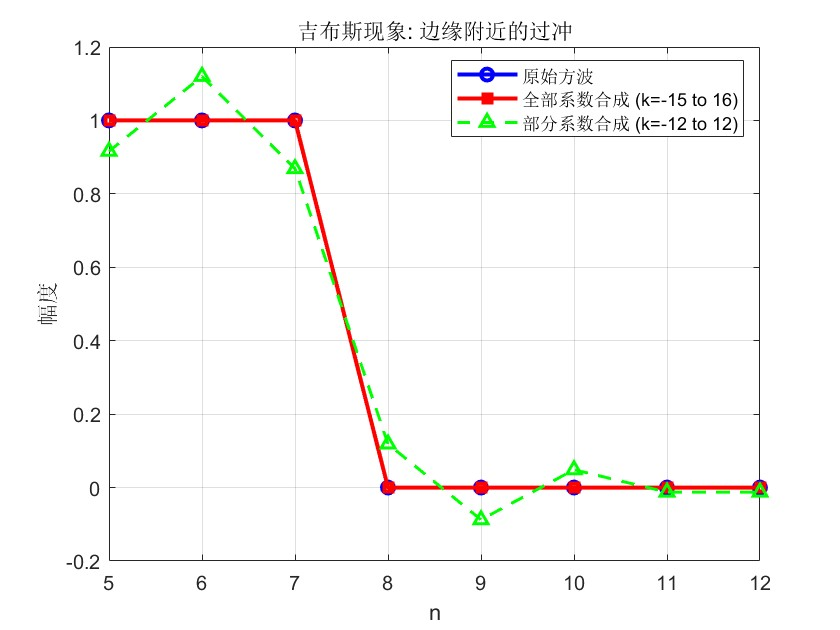
\includegraphics[width=0.8\textwidth]{15.jpg}
\end{figure}


\end{document}